\subsection{Confidence Interval for the Difference Between Two Means}
\label{subsec:conf-inter-for-diff-two-means}

Under the same conditions as in the previous section,
\begin{itemize}
  \item Normal distribution of data or
  \item Sufficiently large sample size,
\end{itemize}
\noindent we can construct a confidence interval for the difference between two means.

\begin{figure}[H]
  \centering
  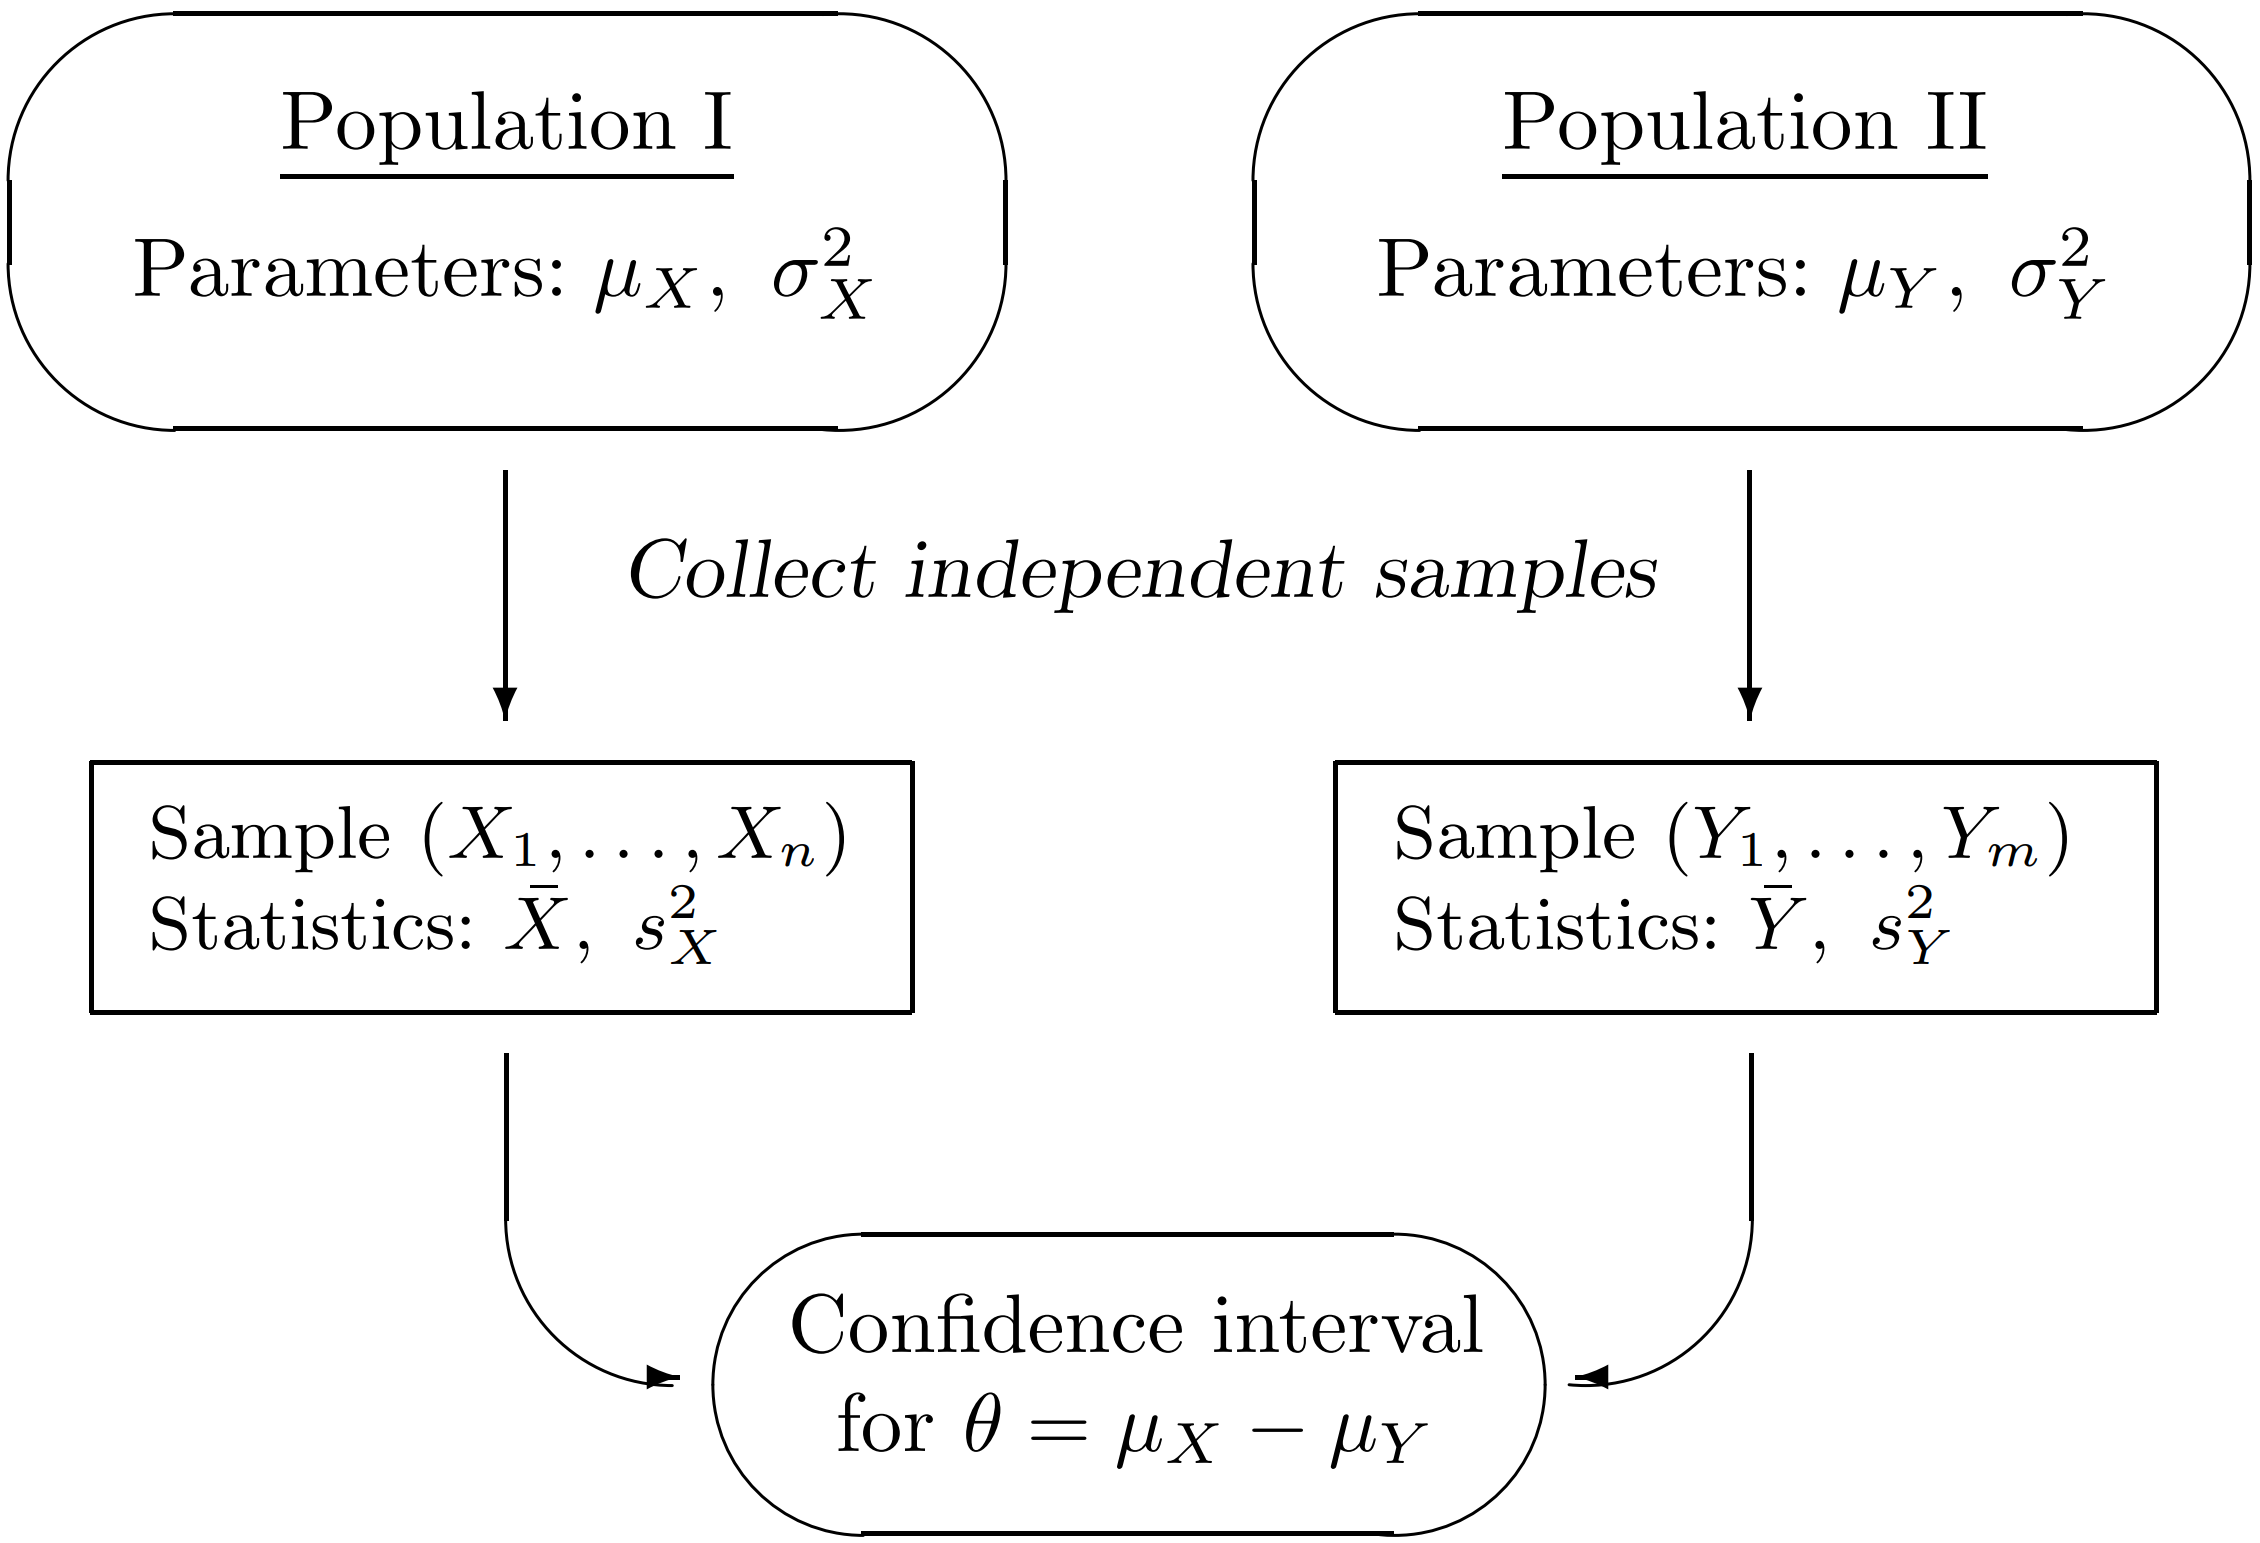
\includegraphics[width=\linewidth]{img/fig-9.4.png}
  \caption{\textit{Comparison of two populations}}
  \label{fig:9.4}
\end{figure}

Suppose that the two samples are collected \textit{independently} of each other. To construct a confidence interval for the difference between population means
\begin{equation*}
  \theta = \mu_X - \mu_Y
\end{equation*}
\noindent we complete the usual steps (a)-(e) below:
\begin{enumerate}[label=(\alph*)]
  \item Propose an estimator of $\theta$,
    \begin{equation*}
      \hat{\theta} = \bar{X} - \bar{Y}
    \end{equation*}
    It is natural to come up with this estimator because $\bar{X}$ estimates $\mu_X$ and $\bar{Y}$ estimates $\mu_Y$.
    \item Check that $\hat{\theta}$ is unbiased. Indeed,
      \begin{equation*}
        \expc{\hat{\theta}} = \expc{\bar{X} - \bar{Y}} = \expc{\bar{X}} - \expc{\bar{Y}} = \mu_X - \mu_Y = \theta
      \end{equation*}
    \item Check that $\hat{\theta}$ has a Normal or approximately Normal distribution. This is true if the observations are Normal or both sample sizes $m$ and $n$ are large.
    \item Find the standard error of $\hat{\theta}$ (using independence of $\bs{X}$ and $\bs{Y}$),
      \begin{align*}
        \sigma(\hat{\theta}) &= \sqrt{\var{\bar{X}} - \var{\bar{Y}}} = \sqrt{\var{\bar{X}} + \var{\bar{Y}}}\\
        &= \sqrt{\frac{\sigma^2_X}{n} + \frac{\sigma^2_Y}{m}}
      \end{align*}
    \item Find quantiles $\pm z_{\alpha/2}$ and compute the confidence interval according to (3). This results in the following formula.
\end{enumerate}
\begin{formula}{Confidence interval for the difference of means; known standard deviations}
  \begin{equation}
    \bar{X} - \bar{Y} \pm z_{\alpha / 2} \sqrt{\frac{\sigma^2_X}{n} + \frac{\sigma^2_Y}{m}}
  \end{equation}
\end{formula}

\begin{example}{ (Effect of an upgrade)}
  A manager evaluates effectiveness of a major hardware upgrade by running a certain process 50 times before the upgrade and 50 times after it. Based on these data, the average running time is 8.5 minutes before the upgrade, 7.2 minutes after it. Historically, the standard deviation has been 1.8 minutes, and presumably it has not changed. Construct a $90\%$ confidence interval showing how much the mean running time reduced due to the hardware upgrade.

  \textbf{Solution:}
  We have $n = m = 50$, $\sigma_X = \sigma_Y = 1.8$, $\bar{X} = 8.5$, and $\bar{Y} = 7.2$. Also, the confidence level $(1 - \alpha)$ equals 0.9, hence $\alpha / 2 = 0.05$, and $z_{\alpha/2} = 1.645$.

  The distribution of times may not be Normal; however, due to large sample sizes, the estimator 
  \begin{equation*}
    \hat{\theta} = \bar{X} - \bar{Y}
  \end{equation*}
  is approximately Normal by the Central Limit Theorem. Thus, formula (6) is applicable, and a $90\%$ confidence interval for the difference of means $(\mu_X - \mu_Y)$ is
  \begin{align*}
    8.5 - 7.2 \pm &1.645 \sqrt{(1.8)^2 \left(\frac{1}{50} + \frac{1}{50}\right)}\\
    &= 1.3 \pm 0.6 \textnormal{ or } \left[ 0.7, 1.9 \right]
  \end{align*}
  We can say that the hardware upgrade resulted in a 1.3-minute reduction of the mean running time, with a $90\%$ confidence margin of 0.6 minutes.
\end{example}

\newpage
